\chapter{Related Work}
\label{chap:lit}

%
%@article{alexopoulou2017task,
%  title={Task effects on linguistic complexity and accuracy: A large-scale learner corpus analysis employing natural language processing techniques},
%  author={Alexopoulou, Theodora and Michel, Marije and Murakami, Akira and Meurers, Detmar},
%  journal={Language Learning},
%  volume={67},
%  number={S1},
%  pages={180--208},
%  year={2017},
%  publisher={Wiley Online Library}
%}
%
%Justifying reliance on NLP tools to process NNS data:
%However, prior studies have shown that native language taggers and parsers perform fairly well on the learner data in EFCAMDAT (Geertzen et al., 2014). For example, Alexopoulou, Geertzen, Korhonen, and Meurers (2015) evaluated the accuracy of extraction of relative clauses, reporting an F score of 83.9%, and found that state-of-the-art NLP tools provide reasonable quality.
%
%#####
%
%
%
%
%@article{papadimitriou2021multilingual,
%  title={Multilingual BERT, Ergativity, and Grammatical Subjecthood},
%  author={Papadimitriou, Isabel and Chi, Ethan A and Futrell, Richard and Mahowald, Kyle},
%  journal={Proceedings of the Society for Computation in Linguistics},
%  volume={4},
%  number={1},
%  pages={425--426},
%  year={2021}
%}
%###
%
%@article{yamazaki2014,
%  title={Toward integrative CALL: A progressive outlook on the history, trends, and issues of CALL},
%  author={Yamazaki, Kasumi},
%  journal={TAPESTRY},
%  volume={6},
%  number={1},
%  pages={6},
%  year={2014}
%}
%"...sociocultural theories of learning, mainly named as Kolb�s (1984) experiential learning and Lave and Wenger�s (1991) situated learning, which emphasize that learning occurs in a communicative context through concrete and direct experiences. Learning in this approach is generally exploratory, thus learners� autonomy, engagement, and, most importantly, motivation are often found to be the most critical elements of contemporary CALL research (cf. Rahimi & Yodollahi, 2011; Ushioda, 2000; Schwienhorst, 2002; Mohammadi, Ghorbani, & Hamidi, 2011; AbuSeileek, 2012)."
%#####
%#####
%@article{collentine2011,
%  title={Learner autonomy in a task-based 3D world and production},
%  author={Collentine, Karina},
%  journal={Language Learning \& Technology},
%  volume={15},
%  number={3},
%  pages={50--67},
%  year={2011},
%  publisher={University of Hawaii National Foreign Language Resource Center}
%}
%With widespread access to technology, learners are increasingly using CALL materials in a learner- centered approach where they take control of their own learning, on their own time, and for their own purposes. These materials include virtual and 3D environments with gaming-like experiences (Darasawang & Reinders, 2010; Sykes, 2009). Highly interactive, multi-sensory environments provide access to real world simulations (Pantelidis, 1993; Schwienhorst, 2008), popularizing online multiuser virtual environments (e.g., Second Life) and massively multiplayer online games (e.g., World of Warcraft). In these autonomous learning environments entailing �independent action� and �decision- making� (Little, 1991, p. 4), it is essential that learners become cognizant of how to learn by raising their metalinguistic awareness and participating in tasks that motivate L2 communication. Fischer (2007) and Schwienhorst (2008) argue that learners in these environments should develop metacognitive abilities, strategies, and have opportunities for reflection (e.g., on input characteristics or their own learning strategies).
%#####
%#####
%@inproceedings{granstrom2004towards,
%  title={Towards a virtual language tutor},
%  author={Granstr{\"o}m, Bj{\"o}rn},
%  booktitle={InSTIL/ICALL Symposium 2004},
%  year={2004}
%}
%In learning a foreign language, visual signals may in many contexts be more important than verbal signals. During the process of acquiring a language, both child L1 speakers and adult L2 speakers rely on gestures to supplement their own speech production (McNeill, 1992; Gullberg, 1998). Adult L2 speakers often make more exten- sive use of gestures than L1 speakers, especially when searching for words or phrases in the new language. In this context, gestures have a compen- satory function in production, often substituting for an unknown word or phrase. L2 listeners may also make greater use of visual cues to aid the conversational flow than do L1 listeners. In this respect, parallels can be made between the situa- tion of the hearing impaired listener and the L2 learner (McAllister 1998).
%It has been found that the integration of seg- mental audio-visual information is affected by the relationship between the language of the speaker and that of the listener. Subjects listening to a for- eign language often incorporate visual informa- tion to a greater extent than do subjects listening to their own language (Kuhl et al. 1994; Burnham and Lau 1999). Furthermore, in a conversation, the L2 learner must not only concentrate on seg- mental phonological features of the target lan- guage while remembering newly learned lexical items, but must also respond to questions at the same time. This task creates a cognitive load for the L2 listener which is in many respects much different from that for the L1 user of a spoken dialogue system. Thus, the compensatory possi- bilities of modality transforms and enhancements of the visual modality are well worth exploring not only concerning segmental, phoneme-level information but also for prosodic and conversa- tional information.
%2 CALL-related projects at CTT
%The CALL research at the Centre for Speech Technology (CTT) focuses on building a Virtual Language Tutor, using an animated talking agent, that addresses these issues, serving as a conversa- tional partner, teacher and an untiring model of pronunciation, who can pick exercises from a training library depending on the user�s needs.
%#####
%#####
%@article{heift2001intelligent,
%  title={Intelligent language tutoring systems for grammar practice},
%  author={Heift, Trude},
%  journal={Zeitschrift f{\"u}r Interkulturellen Fremdsprachenunterricht},
%  volume={6},
%  number={2},
%  year={2001}
%}
%The present paper discusses building a more flexible Web-based grammar practice environment around an Intelligent Language Tutoring System (ILTS). While ILTSs employ Natural Language Processing (NLP) and thus require programming and linguistic expertise, they provide error-specific feedback and flexibility in handling student answers. Sound, graphics and/or videos can also be implemented to achieve a more varied, authentic and contextualized learning environment.
%#####
%#####
%@article{nagata:02,
%	Author = {Noriko Nagata},
%	Date-Added = {2010-08-12 15:04:17 -0400},
%	Date-Modified = {2010-10-19 12:57:46 -0400},
%	Journal = {{CALICO} Journal},
%	Key = {system},
%	Keywords = {ICALL, Japanese},
%	Note = {\url{http://www.usfca.edu/japanese/CALICO02.pdf}},
%	Number = 3,
%	Pages = {583-599},
%	Title = {{BANZAI}: An Application of Natural Language Processing to Web based Language Learning},
%	Volume = 19,
%	Year = 2002}
%
%The BANZAI program, however, is written in Java, which pro- vides excellent support both for sophisticated NLP programming and ap- pealing multimedia applications. As a result, the BANZAI interface is user friendly and visually appealing, making full use of digital photographs, computer graphics, pull down menus, button selections, and Japanese sounds. Each exercise in BANZAI is framed in a conversational setting, along with a relevant photographic or graphical image of Japan, and asks learners to produce a target sentence that is likely to be uttered in real communicative situations.


This dissertation lies at the intersection of several fields including language testing, second language acquisition (SLA), intelligent computer-assisted language learning (ICALL), corpus linguistics and natural language processing (NLP). My work here is much indebted to related research in these areas, and in this chapter I summarize some of the most relevant studies.

%\lk{Maybe it's better to have a P here summarizing my ``ethos'' (low resource, content focused, interpretable) instead of spreading that out below.}

%I begin in Section~\ref{section:ICALLinterp} with a discussion of the importance of transparency and interpretability in ICALL and language testing. In  Section~\ref{section:ICALLoverview}, I examine approaches to ICALL that relate to and inform this dissertation. In Section~\ref{section:learnerCorpora}, I summarize research involving the collection, annotation or content analysis of task-based learner corpora. A brief overview of the NLP tools and methods used in my work is given in Section~\ref{section:NLP}.

%\section{On interpretability for learner applications}
%\label{section:ICALLinterp}
%
%(See also Section~\ref{section:imageProcessing}; this should address the use of sentence encoders like BERT and their use in conjunction with image recognition technology).
%
%This work would be remiss without discussing the role of machine learning (ML) in current NLP, given that such technologies are largely absent from this dissertation. Recent years have seen the rapid development of ML technologies like neural networks and deep learning. \lk{What is ML good at? citations!} These technologies have been widely implemented in areas like NLP and computer vision, often with impressive gains in performance. They can also lead to reductions in the amount of human expertise needed to automate tasks like syntactic labeling, voice recognition and synthesis, and object and facial recognition. \lk{cite stuff} Naturally, this also means significant reductions in the cost of such systems. A major drawback with many such ML technologies, however is the loss of interpretability. For example, \textit{word embeddings} (such as Word2Vec) \lk{cite} are ML based NLP tools suitable for many tasks involving the processing of linguistic meaning or structures. Word2Vec essentially ``learns'' an approximation of the meanings and grammatical usage of words by observing them in context. Instead of relying on expert annotation of features like part-of-speech, sentence structure and morphology to train a model, the system needs only large amounts of raw text. From this text, it observes large numbers of features, such as the average distance between instances of \textit{Word A} and \textit{Word B}. It reduces these raw features to a (still quite large) number of abstract features, or ``latent variables'', which form a vector of numeric values; this vector then serves as a representation of a word's ``meaning''. In a classic example, if one takes the vector for ``queen'', subtracts the vector for ``female'' and adds the vector for ``male'', the resulting vector is roughly equivalent to that of ``king''.
%
%\lk{this is all very cf Brian Riordan's alumni talk... similar sources would be ideal}
%For many applications, the capabilities and cost reduction of ML make it an attractive and suitable choice; this is certainly the case with many NLP tasks. The use of ML tools with learner language is problematic on at least two fronts, however. First, such tools are typically designed for and trained on well-formed, native-like text (or speech). As mentioned, these tools generally do not rely on annotation in their training data; instead, they make up for this lack of expertise by the sheer volume of training data they consume. Including real learner data on the scale required by ML tools would be impractical if not impossible for most researchers. As a result of ML tools' training on mostly native-like data, they are ill-equipped for processing the variability and ambiguity of learner language. For example, native English trained NLP tools expect regular sentence punctuation; text from a beginning English learner lacking in punctuation could therefore be misconstrued as having longer sentences and thus higher proficiency \cite{MeurersDickinson2017}. Second, and perhaps more importantly, tools that rely heavily on ML are inherently less interpretable than ``classical'' NLP tools. Because classical NLP tools are trained on expert annotation, their output is generally determined by the kinds of features that are annotated in the training corpus. This means linguistic researchers can design NLP tools and pipelines that produce output precisely suited for their research questions, so long as they have the resources to produce adequate training corpora. This is not the case with ML based tools, however. Due to their reliance on abstract features and latent variables, these newer tools are largely ``black box'' technologies; raw data goes in and processed data comes out, but even the architect of such a system cannot explain exactly how or why the analysis was produced. In a language learning application, this is problematic because it means the development of a pedagogically sound feedback system for the learner is not possible; the features underlying the analysis are not accessible or interpretable. The outcomes of language testing can have a tremendous impact on a test taker's future, and in such a high stakes application, the lack of interpretability can be even more problematic. Arguably, it is far better for all stakeholders if a language test can deliver not only a score, but also a rationale for that score, such as which kinds of errors a test taker makes and in what contexts. This need for interpretable features was one of a few major factors in the decision to choose classical NLP over newer ML tools in this dissertation, and most of the related studies discussed here take similar approaches.


%\section{Image processing}
%\label{section:imageProcessing}
%This should probably include discussion of ML approaches at image ``encoding/decoding'' and their use in tandem with sentence encoders (BERT, etc.). Ask Ben S. for reading suggestions?
%
%We want to touch on image processing / automatic captioning / use of semantic primatives, etc. -- linguistic annotation of images. NOT a deep discussion, but we need to acknowledge that there are other fields working on the relations between images and text, and give an idea of what some approaches are and how they work, and how they might relate to my work and the work discussed in my lit review.

\section{ICALL}
\label{section:ICALLoverview}
My dissertation project began as an experiment in bootstrapping NLP tools, native speaker data, and learner data to achieve meaning-based  ICALL. I do not attempt a full-fledged ICALL system, but I explore mechanisms for performing the core content analysis that could be implemented in a setting like an ICALL game, an interactive language tutor (ILT) or a language test. I see this work as a push toward pedagogically sound, relatively low-cost, extendable ICALL with an emphasis on content over form. In keeping with this ethos, this section focuses on five ICALL projects that share one or more aspects of my approach, namely the use of existing NLP tools, the processing of free user input (as opposed to menu-based or fill-in-the-blank input), and the use of crowdsourced response models.

\subsection{Herr Kommissar}
\label{section:herr-kommissar}


\textit{Herr Kommissar} \citep{desmedt1991herr,desmedt:95} is an ICALL system for German learners that includes rather robust content analysis and sentence generation. Although it is no longer in use, Herr Kommissar represented significant progress in the integration of communicative and task-based learning in ICALL. The system was styled as a game in which the user plays the role of an American detective traveling through the German countryside who is called upon by local police to help solve murders. To progress through the game and solve mysteries, the user must interview witnesses and interrogate suspects. The user is assisted throughout these dialogs by a local detective. The local detective is effectively the system's feedback agent, providing corrections and recasts of the user's German as well as hints regarding content. In this way, Herr Kommissar set a high bar by cleverly disguising language instruction as realistic communication to create an immersive learning experience and was generally well-received by learners and instructors \cite{harroff1993herr}.

This ICALL system was ambitious and in many ways was ahead of its time---the sentence parsing, sentence generation, language modeling and computing power of the 1990s were not equipped to handle complex discourse. To overcome technical limitations, the system relied on a great deal of hand-built tools, custom decision trees, string matching, and template-based responses that were tailored to the scenario at hand. When users presented off-target or incomprehensible input, the system relied on the assistant detective to redirect conversations, keeping the game ``on the rails'' and maintaining the illusion of authentic conversation. Naturally, these scenario-dependent pipelines were not easily adaptable to new contexts. Nonetheless, Herr Kommissar was a step forward for task-based ICALL and a major inspiration for the work presented throughout this dissertation. In a practical sense, my work started with the goal of enabling an ICALL game like Herr Kommissar using more versatile, plug-and-play NLP techniques.



\subsection{TAGARELA}
\label{section:tagarela}
One relatively well-documented ICALL system is TAGARELA (\textit{Teaching Aid for Grammatical Awareness, Recognition and Enhancement of Linguistic Abilities}), an application for adult learners of Portuguese \cite{amaral2007designing,amaral:meurers:user:07,Amaral.Meurers.Ziai-11}. TAGARELA was developed at The Ohio State University and used by beginning Portuguese learners enrolled there. It relies on a set of NLP modules implemented in a task-based, free input ICALL system. The system includes six different activity types: reading, listening, description, rephrasing, vocabulary and fill-in-the-blank. These different tasks require different types of textual learner input as well as different subsets of the NLP modules for input processing and the generation of feedback.

A crucial component to TAGARELA is its ``Unstructured Information Management Architecture (UIMA),'' which is effectively a collection of text relevant to the tasks that are enriched with multiple annotations relating to both form and meaning. For most tasks, this means TAGARELA relies on a small number of carefully chosen and annotated model responses. This \textit{UIMA} approach means TAGARELA can use a given model in different tasks by varying the NLP pipeline and the selecting the appropriate annotation layers. This approach is also its biggest obstacle, however: each new lesson in TAGARELA requires the careful, deliberate development and testing of expertly annotated model responses. In other words, the system must be ``told'' explicitly what to look for in a user response.

In fairness, TAGARELA was not designed to be a fully-fledged ICALL system ready for widespread use, but rather as an experiment and a data collection tool for ICALL researchers, and in this regard, it stands as a successful project and an important step toward handling meaning in ICALL with cleverly-implemented NLP. Prior to any system development, the TAGARELA team began their work with the creation of a ``taxonomy of expected errors,'' gleaned from an analysis of a corpus of written assignments from learners of Portuguese. The authors describe this development approach as ``data-driven rather than process-driven''. This bucks a tendency among many ICALL developers to simply address the kinds of errors NLP tools can readily identify. 
%\lk{cite DuoLingo? etc.}
%What is needed instead is ICALL development informed by SLA research and by the kinds of challenges learners face, as borne out by real data.
%\lk{cite Ellis, Meurers}
The errors annotated in the Portuguese learner data and handled by TAGARELA cover both form and meaning, with error types consisting of, for example, \textit{spelling}, \textit{agreement} and \textit{word choice}.
My work was inspired by TAGARELA's data-driven approach, and especially by its prioritization of the handling of errors related to meaning. Moreover, TAGARELA demonstrated for ICALL the successful use of ordinary and interpretable NLP tools---primarily a tokenizer, part of speech tagger and syntactic parser.

\subsection{E-Tutor}
\label{section:e-tutor}
\cite{heift2010}
%
%For instance, the activity types in the E-Tutor (Heift, 2010b)
%allow for grammar practice as well as reading comprehension and/or cultural knowledge
%and also supports discovery learning in the form of exploration of learner language. For
%this, user submissions over five years were compiled and from those a common learner
%corpus was constructed that allows students to explore learner language according to
%various parameters. Thus, learners can examine interlanguage or task-specific phenomena
%and the benefits in this respect have been well documented (Granger, 2003a). Moreover, 
%these large data sets also allow language instructors and/or researchers to examine the
%design of language learning material in addition to a wide range of additional research
%topics (e.g., use of help options, interlanguage studies).
%Similarly, Robo-Sensei developed by Nagata (2009) for L2 learners of Japanese
%analyses student input for selected exercises, performs an itemization (separating tokens
%for later linguistic analysis) and a morphological analysis, and parses the sentential input
%syntactically using a context-free grammar. Finally, Tagarela (Amaral \& Meurers, 2011)
%an ICALL system for Portuguese is similar to the E-Tutor and RoboSensei, in that it uses
%the metaphor of an electronic textbook. The system provides practice with grammar and
%listening comprehension and students receive feedback on spelling, morphological,
%syntactic and semantic errors. These three systems are used in the regular L2 language
%classroom.


\subsection{Robo-Sensei}
\label{section:robo-sensei}
\cite{nagata2009robo}

\subsection{C-Rater, etc.}
\label{section:c-rater}
\cite{leacock:chodorow:03}

\cite{somasundaran:chodorow:14}

\cite{somasundaran:ea:15}


%
%
%\bigskip
%NOTES:
%\bigskip
%
%for the wide range of language activities supporting significant well-formed
%or ill-formed variation of form, meaning, or task-appropriateness of learner responses, it is
%necessary to abstract away from the specific string entered by the learner to more general
%classes of properties by automatically analyzing the learner input using NLP algorithms and
%resources.
%
%...
%
%Nagata, N. (2009). Robo-Sensei�s NLP-Based Error Detection and Feedback Generation.
%CALICO Journal 26(3), 562�579. URL http://purl.org/calico/nagata09.pdf.
%
%Nagata (2009, pp. 563f) provides a clear illustration of this with an exercise taken from her
%Japanese tutor ROBO-SENSEI in which the learner reads a short communicative context and
%is asked to produce a sentence in Japanese that is provided in English by the system. The
%learner response in this exercise is directly dependent on the input provided by the exercise
%(a direct response in the terminology of Bachman \& Palmer, 1996), so that a short, seven
%word sentence can be defined as target answer. Yet after considering possible well-formed
%lexical, orthographic, and word order variants, one already obtains 6048 correct sentences
%which could be entered by the learner. Considering incorrect options, even if one restricts
%ill-formed patterns to wrong particle and conjugation choices, one obtains almost a million
%sentences.
%
%...
%
%Complementing the analysis of form, for an ILTS to offer meaning-based, contextualized ac
%tivities
%it is important to provide an automatic analysis of meaning aspects, e.g., to determine
%whether the answer given by the learner for a reading comprehension question makes sense
%given the reading.
%



%\section{Learner corpora}
%\label{section:learnerCorpora}
%Here I will discuss task-based learner corpora research that relates to my work. This includes discussions of task design, data collection, annotation schemes, and automatic processing. I focus in particular on the learner content analysis research conducted by two clusters of researchers: one primarily associated with The Ohio State University and consisting of Detmar Meurers and colleagues, and the other primarily associated with Educational Testing Services (ETS) and consisting of Martin Chodorow, Swapna Somasundaran and Joel Tetrault and colleagues. 
%
%Here are some papers I discussed briefly in my BEA 2018 paper:
%
%\cite{leacock:ea:14}
%
%\cite{kyle2015automatically}
%
%\cite{weigle2013english}
%
%\cite{amaral:meurers:user:07}
%
%\cite{Meurers.Dickinson-17}
%
%\cite{heift:schulze:07}
%
%\cite{somasundaran:ea:15}
%
%\cite{bailey:meurers:08}
%
%\cite{meurers2011evaluating}
%
%\cite{somasundaran:chodorow:14}
%
%\cite{cahill-et-al:14}
%
%\cite{ragheb:dickinson:14a}
%
%\cite{foster2009native}
%
%\cite{cho2013investigating}
%
%\cite{landis1977measurement}
%
%\cite{artstein:massimo:2008}
%
%\cite{tetreault-chodorow:2008:HJCL}
%
%\cite{tetreault:chodorow:08}
%
%\section{Language assessment}
%\label{section:languageAssessment}
%
%\section{NLP tools and methods}
%\label{section:NLP}
%
%\section{My previous work}
%\label{section:myPreviousWork}
%Here I will discuss the work I have previously done in this area, including the papers given in the subsections below.
%
%\subsection{2013}
%\cite{king:dickinson:13}
%
%\begin{figure}
%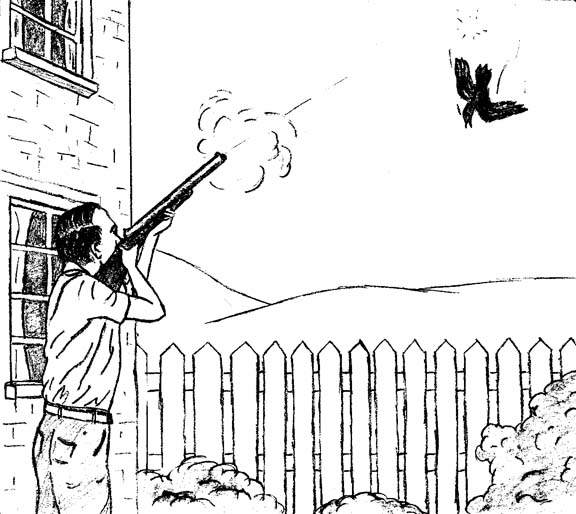
\includegraphics[width=.7\textwidth]{figures/exampleprompt2.jpg}
%\caption{This is an example figure from \citet{king:dickinson:13}.}
%\label{figure:KandD2013}
%\end{figure}
%
%\subsection{2014}
%\citet{king:dickinson:14}
%
%\subsection{2016}
%\citep{king:dickinson:16}
%
%\subsubsection{Bag-of-dependencies}
%Here we could discuss the switch to a bag-of-dependencies approach, the use of tf-idf and the use of vector cosine distance for ranking responses.
%
%\subsubsection{Clustering}
%Here we could briefly mention the clustering experiments we did in the 2016 paper. But really, I'd rather not, because I don't intend to repeat them in the dissertation.
%
%\subsection{2018}
%\cite{king:dickinson:18}
%
%\begin{figure}
%
\includegraphics[width=.7\textwidth]{figures/I29.jpg}
%\caption{This is an example figure from \citet{king:dickinson:18}.}
%\label{figure:KandD2018}
%\end{figure}


% This is a figure in landscape orientation
%\begin{sidewaysfigure}
%
\includegraphics[width=\textwidth]{figures/exampleFigure.png}
%\caption{This is another example Figure, rotated to landscape orientation.}
%\label{LandscapeFigure}
%\end{sidewaysfigure}

%While there is much current work on analyzing learner language, it
%usually focuses on grammatical error detection and correction
%\citep[e.g.,][]{HOO2012} and less on semantic analysis.  At the same
%time, Intelligent Computer-Assisted Language Learning (ICALL) and
%Intelligent Language Tutoring (ILT) systems
%\citep[e.g.,][]{heift:schulze:07, meurers:12} also tend to focus more
%on grammatical feedback. An exception to this rule is \textit{Herr
%  Komissar}, an ILT for German learners that includes rather robust
%content analysis and sentence generation \citep{desmedt:95}, but this
%involves a great deal of hand-built tools and does not connect to
%modern NLP.  Some work addresses content assessment for short answer
%tasks \citep{Meurers.Ziai.ea-11}, but this is still far from naturalistic,
%more conversational interactions \citep[though, see][]{petersen:10}.
%
%Our overarching goal is to facilitate ILTs and language assessment tools that maximize free
%interaction, building as much as possible from existing NLP resources.
%While that goal is in the distant future, the more immediate goal in
%this paper is to pinpoint the precise challenges which interactive
%learner sentences present to constructing semantic analyses, even when
%greatly constrained.  We approximate this by collecting data from a
%task which models some aspects of interaction, namely a picture
%description task (PDT), parsing it with an off-the-shelf parser,
%extracting semantic forms, and noting the challenges throughout.
%
%The focus towards interaction is in accord with contemporary theory
%and research in Second Language Acquisition (SLA) and best practices
%in second language instruction, which emphasize the limiting of
%explicit grammar instruction and feedback in favor of an approach that
%subtly integrates the teaching of form with conversation and
%task-based learning \citep{CelceMurcia:1991:GrammarPedagogy,
%  CelceMurcia:2002:GrammarThroughContext,
%  LarsenFreeman:1991:TeachingGrammar}.  Indeed,
%\citet{Ellis:2006:CurrentIssues} states, ``a traditional approach to
%teaching grammar based on explicit explanations and drill-like
%practice is unlikely to result in the acquisition of the implicit
%knowledge needed for fluent and accurate communication.''  For our
%purposes, this means shifting the primary task of an ICALL application
%from analyzing grammar to evaluating semantic appropriateness and
%accuracy.
%
%The data for error detection work is ideal for developing systems
%which provide feedback on essays, but not necessarily for more
%interactive communication.  Thus, our first step is to collect data
%similar to what we envision processing in something like an ILT game,
%data which---as far as we know---does not exist.  While we desire
%relatively free production, there are still constraints; for games,
%for example, this comes in the form of contextual knowledge (pictures,
%rules, previous interactions).  To get a handle on variability under a
%set of known constraints and to systematically monitor deviations from
%target meanings, we select a PDT as a constrained task that still
%promotes interactive communication.
%Collecting and analyzing this data is our first major contribution, as
%described in section~\ref{sec:data}.
%
%Once we have the data, we can begin to extract semantic forms, and our
%second major contribution is to outline successes and pitfalls in
%obtaining shallow semantic forms in interactive learner data, as
%described in section~\ref{sec:method}, working from existing tools.
%Although we observe a lot of grammatical variation, we will
%demonstrate in section~\ref{sec:evaluation} how careful selection of
%output representations (e.g., the treatment of prepositions) from an
%off-the-shelf parser and a handful of syntax-to-semantics rules allow
%us to derive accurate semantic forms for most types of transitive verb
%constructions in our data.  At the same time, we will discuss the
%difficulties in defining a true gold standard of meanings for such a
%task.  Finally, we examine methods for automatically correcting misspellings, showing that preprocessing with spelling correction tools and language modeling can significantly reduce downstream errors. This work paves the way for increasing the range of
%constructions and further exploring the space between free and
%constrained productions \citep[see also the discussion
%in][]{Amaral.Meurers-11}.

%\section{Related Work}
%
%In terms of our overarching goals of developing an interactive ILT,
%a number of systems exist (e.g., TAGARELA
%\citep{Amaral.Meurers.Ziai-11}, e-Tutor \citep{heift:01}), but few
%focus on matching semantic forms.  \textit{Herr Komissar}
%(\citet{desmedt:95}) is one counter-example; in this game, learners
%take on the role of a detective tasked with interviewing suspects and
%witnesses. The system relies largely on a custom-built database of
%verb classes and related lexical items. Likewise, \citet{petersen:10}
%designed a system to provide feedback on questions in English,
%extracting meanings from the Collins parser \citep{collins:99}.  Our
%work is is in the spirit of his, though our starting point is to
%collect data of the type of task we aim to analyze, thereby
%pinpointing how one should begin to build a system.
%
%The basic semantic analysis in this paper parallels work on content
%assessment (e.g., ETS's c-rater system
%\citep{leacock:chodorow:03}).  Different from our task, these systems
%are mostly focused on essay and short answer scoring, though many focus on semantic
%analysis under restricted conditions. As one example,
%\citet{Meurers.Ziai.ea-11} evaluate English language learners' short
%answers to reading comprehension questions, constrained by the topic
%at hand. Their approach performs multiple levels of annotation on the
%reading prompt, including dependency parsing and lexical analysis from
%WordNet \citep{Fellbaum:1998}, then attempts to align elements of the
%sentence with those of the (similarly annotated) reading prompt, the
%question, and target answers to determine whether a response is
%adequate or what it might be missing.  Our scenario is based on
%images, not text, but our future processing may need to
%include similar elements, e.g., determining lexical relations from
%WordNet.
%


